\documentclass[12pt,a4paper]{amsart}

% ukazi za delo s slovenscino -- izberi kodiranje, ki ti ustreza
\usepackage[slovene]{babel}

%\usepackage[T1]{fontenc}
\usepackage[utf8]{inputenc}
\usepackage{amsmath,amssymb,amsfonts}
\usepackage{url}
%\usepackage[normalem]{ulem}
\usepackage[dvipsnames,usenames]{color}
\usepackage{verbatim}

\usepackage{graphicx}
\graphicspath{ {./images/} }



% ne spreminjaj podatkov, ki vplivajo na obliko strani
\textwidth 15cm
\textheight 24cm
\oddsidemargin.5cm
\evensidemargin.5cm
\topmargin-5mm
\addtolength{\footskip}{10pt}
\pagestyle{plain}
\overfullrule=15pt % oznaci predlogo vrstico


% ukazi za matematicna okolja
\theoremstyle{definition} % tekst napisan pokoncno
\newtheorem{definicija}{Definicija}[section]
\newtheorem{primer}[definicija]{Primer}
\newtheorem{opomba}[definicija]{Opomba}

\renewcommand\endprimer{\hfill$\diamondsuit$}


\theoremstyle{plain} % tekst napisan posevno
\newtheorem{lema}[definicija]{Lema}
\newtheorem{izrek}[definicija]{Izrek}
\newtheorem{trditev}[definicija]{Trditev}
\newtheorem{posledica}[definicija]{Posledica}


% za stevilske mnozice uporabi naslednje simbole
\newcommand{\R}{\mathbb R}
\newcommand{\N}{\mathbb N}
\newcommand{\Z}{\mathbb Z}
\newcommand{\C}{\mathbb C}
\newcommand{\Q}{\mathbb Q}

% ukaz za slovarsko geslo
\newlength{\odstavek}
\setlength{\odstavek}{\parindent}
\newcommand{\geslo}[2]{\noindent\textbf{#1}\hspace*{3mm}\hangindent=\parindent\hangafter=1 #2}

% naslednje ukaze ustrezno popravi
\newcommand{\program}{Matematika z računalnikom} % ime studijskega programa: Matematika/Finan"cna matematika
\newcommand{\imeavtorja}{Jan Založnik in Mai Praskalo} % ime avtorja
\newcommand{\imementorja}{} % akademski naziv in ime mentorja
\newcommand{\naslovdela}{}
\newcommand{\letnica}{2022} %letnica diplome


% vstavi svoje definicije ...




\begin{document}

% od tod do povzetka ne spreminjaj nicesar
\thispagestyle{empty}
\noindent\large
UNIVERZA V LJUBLJANI\\[3mm]
FAKULTETA ZA MATEMATIKO IN FIZIKO\\[2mm]
% FAKULTETA ZA RAČUNALNIŠTVO IN INFORMATIKO\\[2mm]
GEN-I\\[5mm]
% \program\ -- 2.~stopnja}
\vfill

\begin{center}{\large
\imeavtorja\\[2mm]
% {\bf \naslovdela}\\[10mm]
{\bf Uporaba metod strojnega učenja za napoved gibanja cen posameznih urnih blokov}\\[1cm]
%Mentor: \imementorja}
}
\end{center}
\vfill

\noindent{\large
Ljubljana, \letnica}

\pagebreak
\tableofcontents
\listoffigures
\pagebreak

\section{Motivacija}

Električno energijo je v primerjavi z ostalimi energenti in dobrinami zelo zahtevno shranjevati, 
zato morata biti proizvodnja in poraba električne energije konstantno v ravnovesju.
Tržni igralci tako izravnavajo svojo proizvodnjo in porabo na znotrajdnevnih trgih električne energije,
kjer se trguje elektrika za dobavo v posameznih 15 minutnih blokih do vsega nekaj minut pred začetkom 
dobave. V zadnjih letih se je predvsem zaradi rasti deleža proizvodnje elektrike iz obnovljivih virov, 
ki je zaradi odvisnosti od vremena težko napovedljiva, dejavnost na znotrajdnevnih trgih močno povečala, 
igralci na teh trgih pa vedno večji delež odločitev prepuščajo umetni intelegenci.



\section{Opis naloge}

Pri nalogi bova s pomočjo metod strojnega učenja napovedala gibanje cen posameznih urnih
 blokov. Pri tem bova uporabila pretekle podatke o gibanju cen elektrike kot tudi ostalih energentov, 
 vremenske napovedi različnih ponudnikov, podatke o proizvodnji različnih elektrarn itd. 

Najina glavna naloga je ustvariti program, ki bo sprejel zgodovinske podatke o vremenu, cene posameznih
 blokov dnevnega (angl. \textit{day-ahead}) trga ter cene drugih energentov in bo s pomočjo teh poskušal čim bolje napovedati ceno na pripadajočem znotraj dnevnem (angl. \textit{intra-day}) trgu. 
 Za začetek bova opravila analizo podatkov, cena iz dnevnega trga predstavlja že nek začetni približek cen na znotraj dnevnem trgu, zato bova to vzela kot osnovno napoved, ki jo bova skušala izboljšati.



\section{Električni trg v Evropi}

V ekonomskem smislu je elektrika surovina, s katero je mogoče trgovati na trgu električne energije \textbf{PX} (angl. \textit{Power Exchange}). Kot je že bilo omenjeno je električno energijo zelo težko shranjevati in hkrati morata biti proizvodnja in poraba neprestano v ravnovesju.
 Na trgu dobimo pošteno ceno z načelom ponudbe in povpraševanja, kar pomeni, da proizvajalci podajo ponudbo (koliko električne energije lahko proizvedejo in za kakšno ceno), nasprotno porabniki električne energije podajo povpraševanje (koliko električne energije bodo porabili in koliko so zanj pripravljeni plačati). 
Tako dobimo dve krivulji in stičišče teh predstavlja ceno elektrike, kar prikazuje slika \ref{fig:postena_cena}. Zavedati se moramo, da so na trgu mogoče tudi negativne cene.
 Negativne cene so cenovni signal na veleprodajnem trgu električne energije, ki se pojavi, ko visoka nefleksibilna proizvodnja električne energije zadovolji nizko povpraševanje. Neprilagodljivih virov energije ni mogoče hitro in stroškovno učinkovito izklopiti in znova zagnati. Prav tako je cenovno zahtevno zaustaviti obnovljive vire energije.  
 Cene padajo z nizkim povpraševanjem in signalizirajo generatorjem na zmanjšanje proizvodnje, da se izognejo preobremenitvi omrežja. Na dnevnem in znotraj dnevnem trgu lahko tako cene padejo pod ničlo.

\begin{figure}[h]
    \centering
    \includegraphics[scale=0.75]{curve}
    \caption{Graf ponudbe in povpreševanja}
    \label{fig:postena_cena}
\end{figure}


V Evropi imamo več različnih električnih trgov, največja sta Nord Pool (v 16 državah) in Epex Spot (v 13 državah), vendar Slovenija ni del nobenega od teh. 
Povezovanje evropskih trgov omogoča prost pretok električne energije čez meje, kar poveča konkurenčnost na trgu ter s tem dosežemo boljšo učinkovitost. S čezmejnim trgovanjem torej vplivamo na socialno blaginjo vseh Evropejcev.
V najini nalogi se bova osredotočila le na Nemčijo, ki je del obeh izmed omenjenih trgov. Prav tako so bile na teh trgih izvedene vse transakcije o trgovanju, 
ki jih bova uporabila pri analizi in napovedovanju. 


Evropska Unija se zavzema, da se bo delež obnovljivih virov do leta 2030 dvignil iz 25\% na več kot 50\%. Prav tako je cilj, da bodo proizvedli zadostno količino energije tudi ko ne bo vetra ali sonca. 
Eden izmed načinov je shranjevanje električne energije, ko veterne in sončne elektrarne pridelajo presežek. 



\section{Dnevni in znotraj dnevni trg}

Dnevni trg se upravlja prek dražbe, ki poteka enkrat na dan, skozi celotno leto. Na tej dražbi se trguje za vse ure naslednjega dne. Naročila so prijavljena s strani udeležencev na trgu, 
in sicer imajo udeleženci čas do 12:00 UTC, da oddajo vsa ponudbe in povpraševanja za naslednji dan. Na podlagi nakupnih naročil se vzpostavi krivulja povpraševanja, na podlagi prodajnih naročil pa krivulja ponudbe za vsako uro naslednjega dne. Tržna klirinška cena (MCP), ki odraža ponudbo in povpraševanje, leži na presečišču obeh krivulj.


Na znotraj dnevnem trgu udeleženci trgujejo neprekinjeno, 24 ur na dan, z dostavo še isti dan. Takoj, ko se ujemata naročilo za nakup in prodajo, se posel izvede. Z električno energijo je mogoče trgovati do 5 minut pred dostavo in prek urnih, polurnih ali četrturnih pogodb. Ker to omogoča visoko stopnjo prilagodljivosti, člani uporabljajo znotraj dnevni trg za prilagoditve v zadnjem trenutku in za uravnoteženje svojih pozicij bližje dejanskemu času. Čezmejno trgovanje je bistveno pri trgovanju znotraj dneva. 


% \begin{comment}
\section{Nemčija}

Nemčija se je zavezala, da bo do leta 2020 zmanjšala emisije toplogrednih plinov za 40 \% v primerjavi iz leta 1990 in za 80–85 \% do leta 2050 glede na raven iz leta 1990. Da bi cilj lahko dosegli, načrtujejo preoblikovanje svojega sistema oskrbe z električno energijo, ki bo v celoti temeljila na obnovljivih virih energije. 
Potencial za zmanjšanje emisij v elektroenergetskem sektorju je zelo velik, saj ima energetski sektor ključno funkcijo glede emisij toplogrednih plinov, saj trenutno povzroča več kot 80 \% emisij v Nemčiji in znotraj tega sektorja je oskrba z električno energijo odgovorna za približno 40 \% emisije CO2, povezane z energijo. 
Z visoko učinkovito rabo električne energije, ki bi v celoti temeljila na obnovljivih virih energije, bo mogoče doseči skoraj nič emisij toplogrednih plinov.
Zanimiva je tudi porazdelitev nemških električnih virov, ki je prikazana na sliki \ref{fig:distribution}. Hitro se lahko opazi, da velik delež predstavljata veterna in sončna energija, ki pa sta seveda zelo odvisna od vremena.
% \end{comment}

% \begin{comment}
\begin{figure}[h]
    \centering
    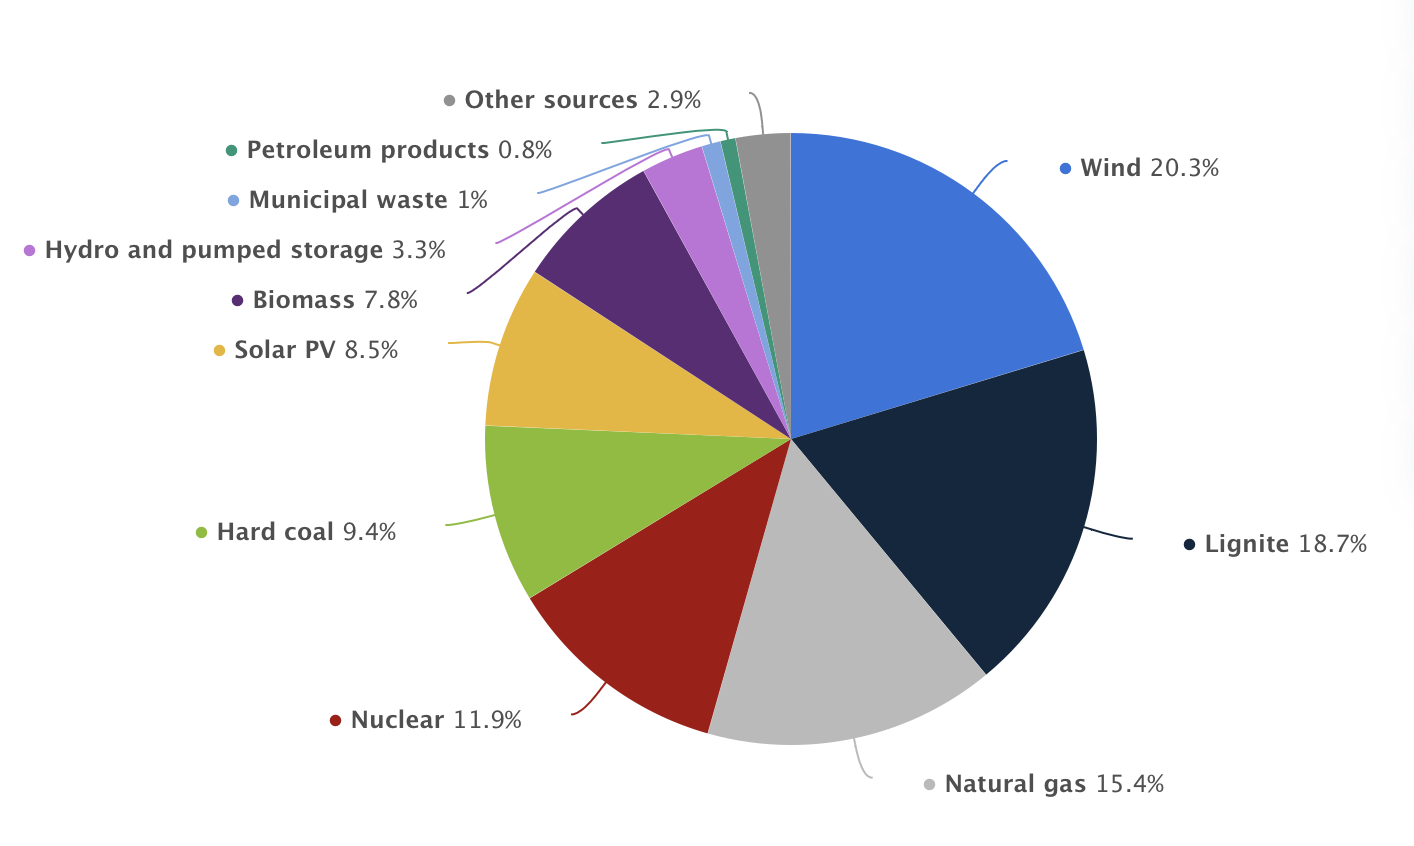
\includegraphics[scale=0.5]{porazdelitev_germany_2021.png}
    \caption{Porazdelitev nemških električnih virov v letu 2021}
    \label{fig:distribution}
\end{figure}
% \end{comment}


\section{Vremenski podatki}

Vremenske podatke sva pridobila iz Evropskega centra za vremenske napovedi (ECMWF). Kot sva že omenila, bo imelo vreme zaradi vedno večjega deleža obnovljivih virov vedno večji vpliv na cene in proizvajanje elektrike. 
Največji delež obnovljivih virov sta v letu 2021 predstavljala veter in sončna energija, zato sva za napoved proizvedene energije pridobila veterne in sončne napovedi iz ECMWF. 

Da bi bila ocena čim bolj natančna sva upoštevala dejstvo, da je na posameznih delih Nemčije veliko več veternih elektrarn (Slika \ref{fig:veter}). 
Podatke o hitrosti vetra sva nato pridobila za vsako zvezno državo, in sicer sva pri vsaki upoštevala zmogljivost elektrarn in vzela povprečje 25 najbližjih geografskih točk.
Iz dejanskih podatkov cen produktov na trgu in podatkov o hitrosti vetra, sva ugotovila da obstaja približno 20\% negativna korelacija med ceno prouktov in hitrostjo vetra. Torej 
če je veter močnejši proizvede več električne energije in tako vpliva na znižanje cene električne energije. 

Vendar sva se zaradi omejene količine napovednih podatkov, ki sva jih lahko pridobila iz ECMWF, odločila, da bova za nadalnje delo uporabljala vetrne podatke, ki sva jih dobila s strani GEN-I. 
Tako sva dobila veliko boljše vremenske napovedi, ki so hkrati že pretvorjeni v potencialno pridelavo električne energije. S tem sva tako dobila napovedi v razmiku 15 minut, kar je veliko boljše od razmika podaktov, ki sva jih pridobila sama, in sicer je bil tam najmanjši razmik 6 ur.  


Sončne elektrarne so porazdeljene bolj enakomerno (slika \ref{fig:sonce}). Vendar zopet niso bili napovedni podatki dovolj dobri, da bi jih lahko uporabila pri napovedi, zato sva tudi te podatke morala naposled dobiti od GEN-I. Zopet sva dobila podatke, ki so že pretvorjeni v potencialno električno energijo.




% \begin{comment}
\begin{figure}[h]
    \centering
    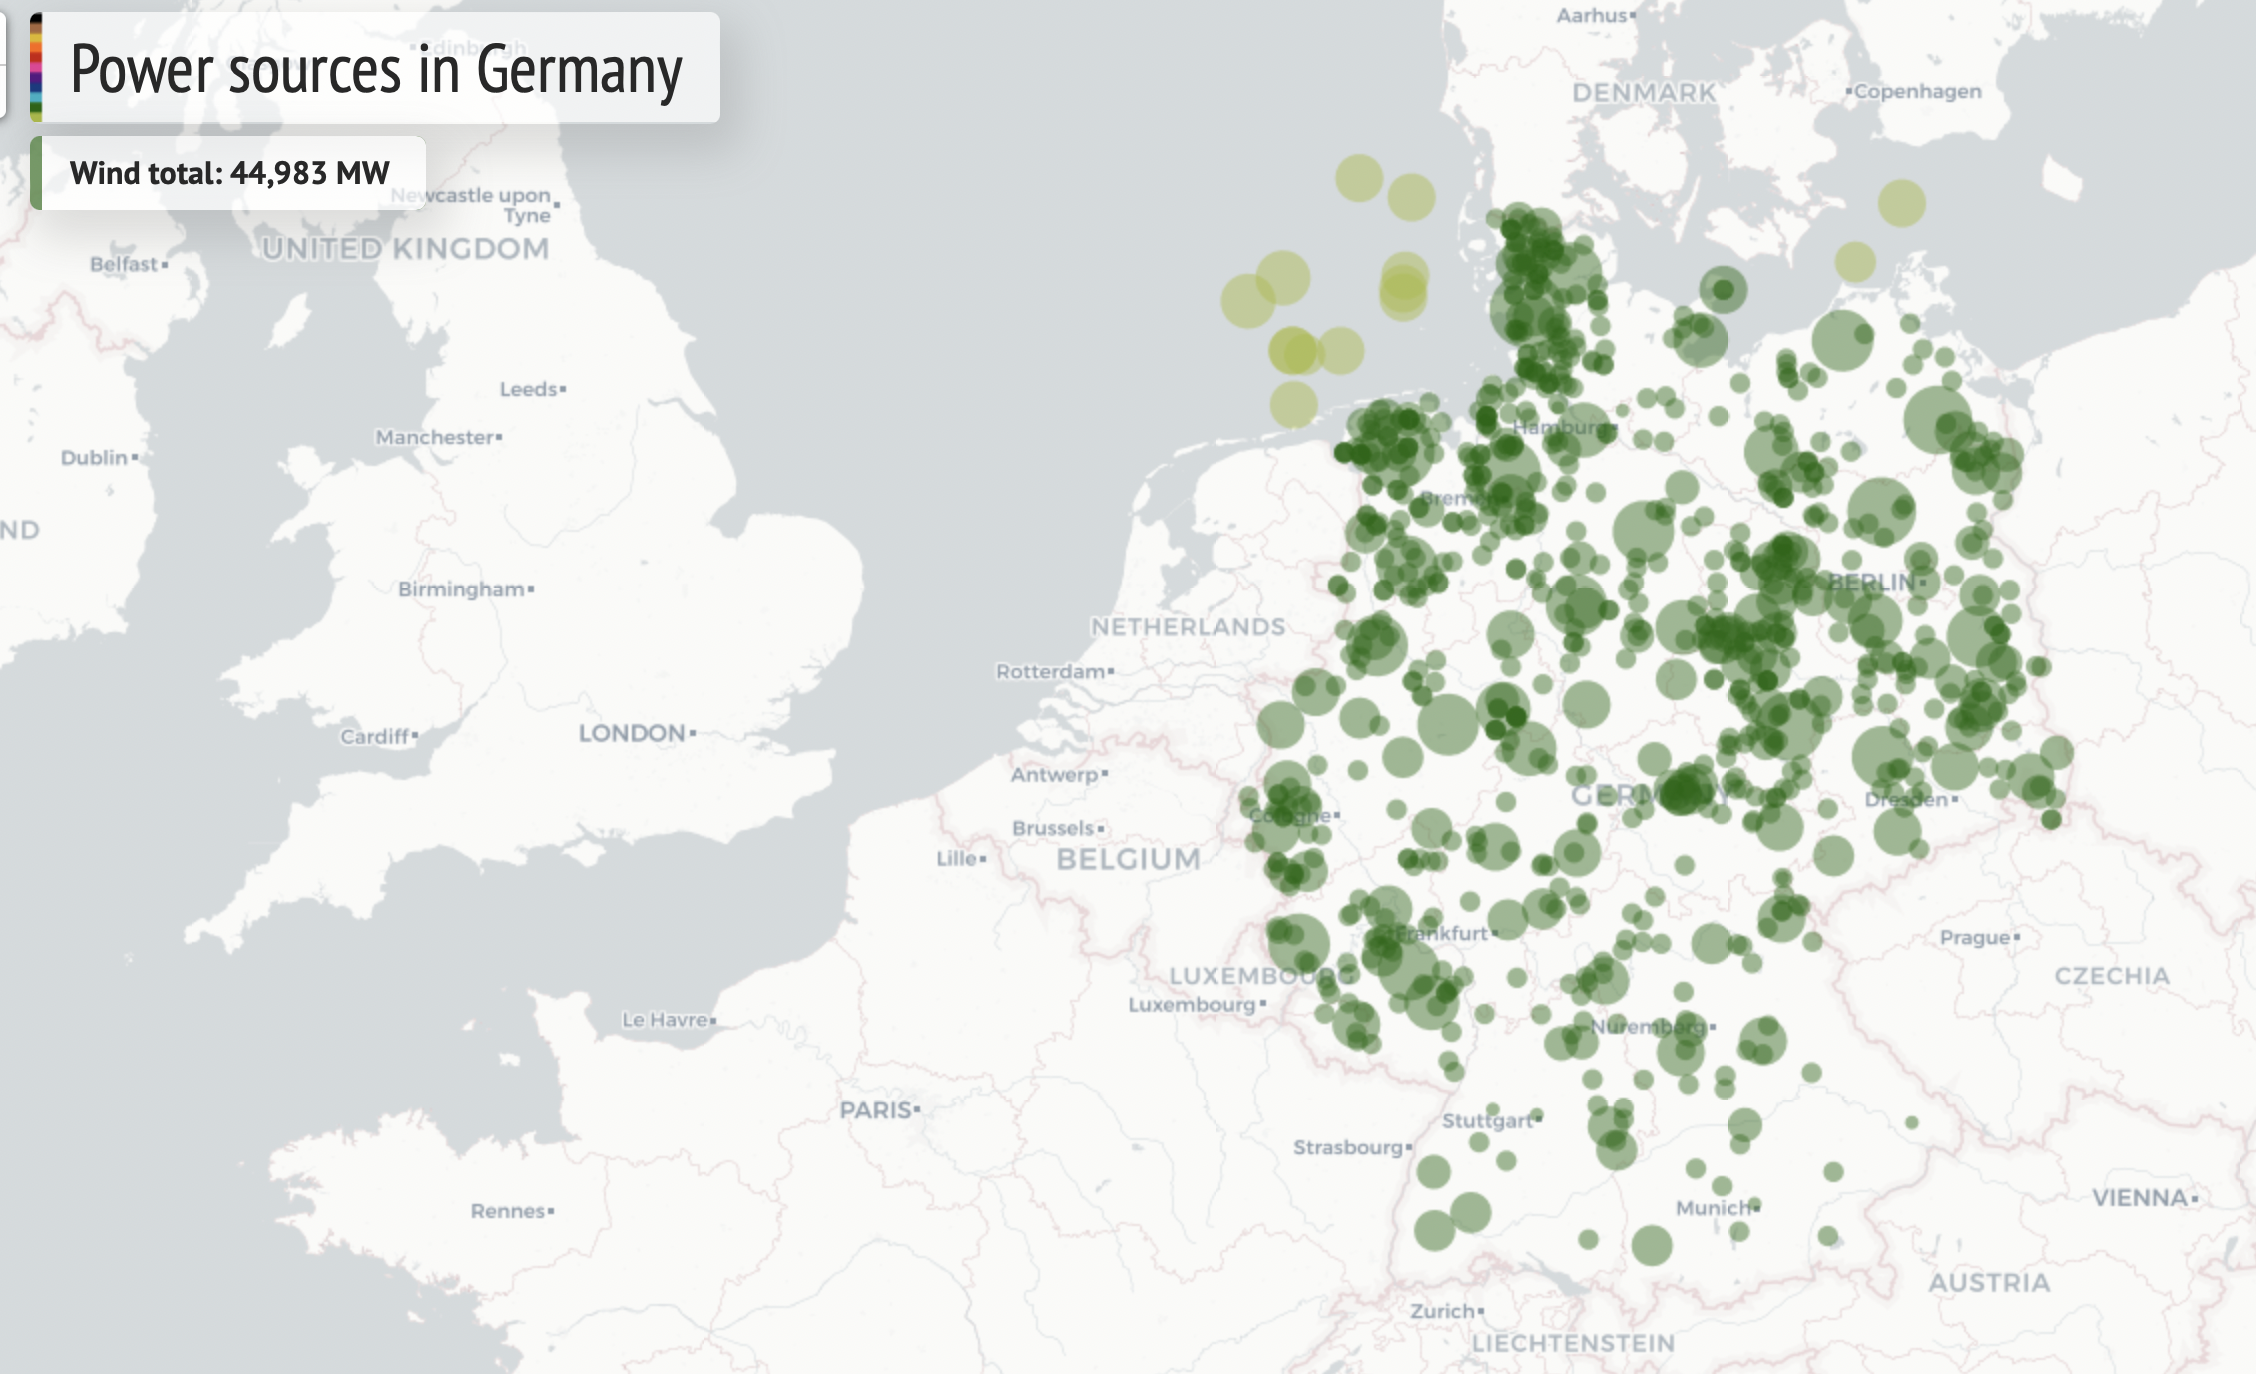
\includegraphics[scale=0.35]{wind_2016.png}
    \caption{Vetrne elektrarne v Nemčiji}
    \label{fig:veter}
\end{figure}

\begin{figure}[h]
    \centering
    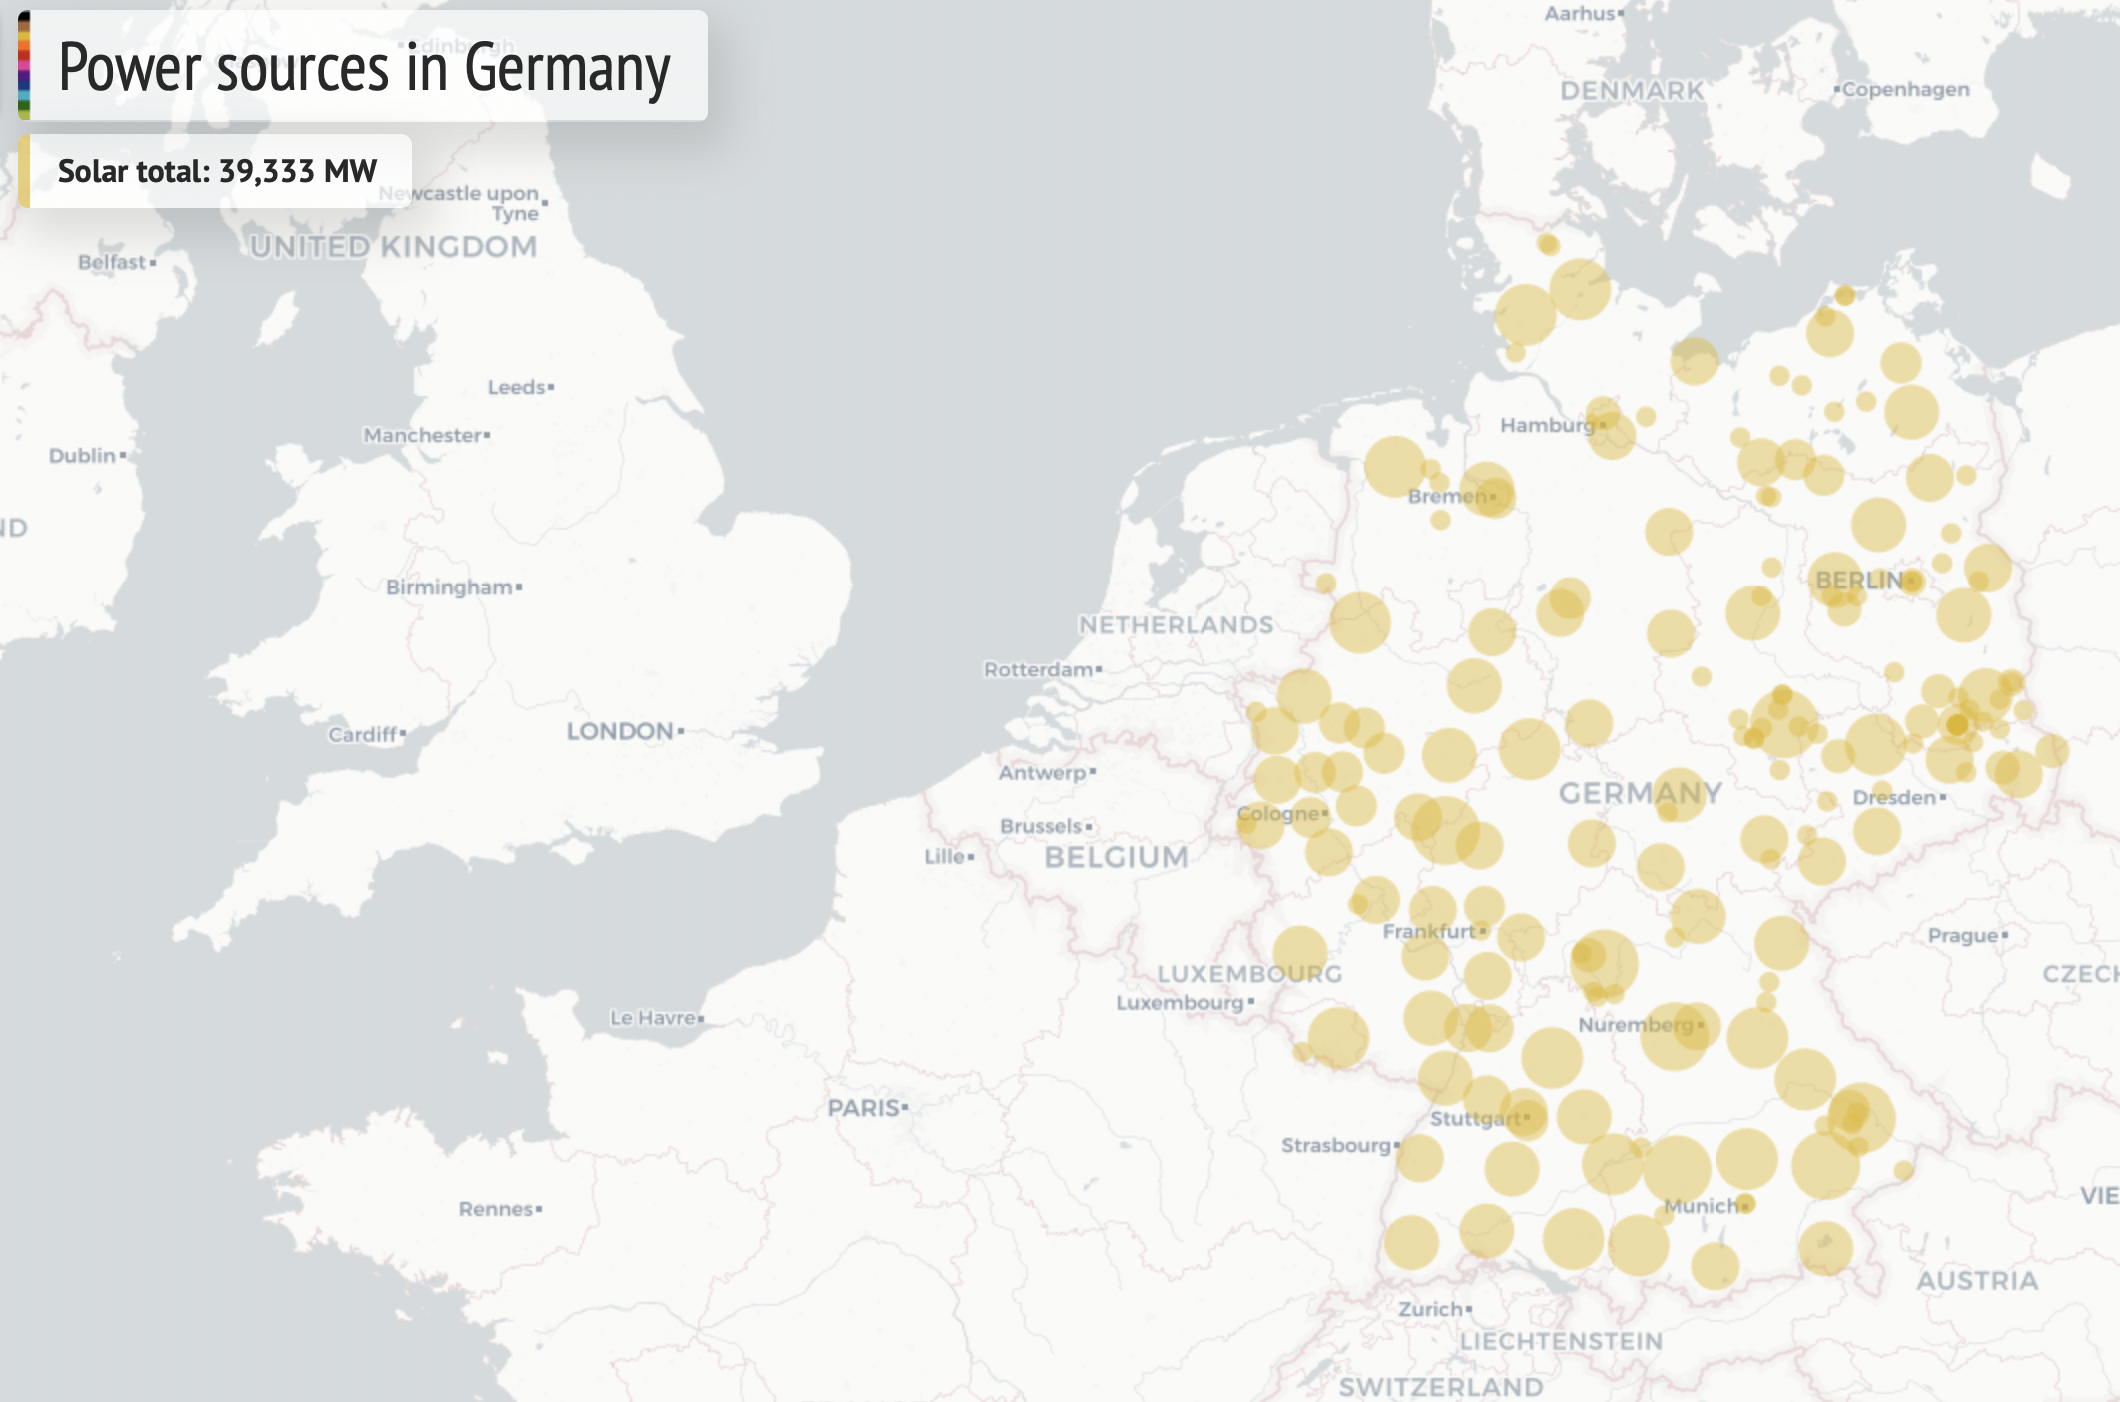
\includegraphics[scale=0.35]{solar_2016.png}
    \caption{Sončne elektrarne v Nemčiji}
    \label{fig:sonce}
\end{figure}
% \end{comment}



% linki:

% https://www.carbonbrief.org/how-germany-generates-its-electricity

%\subsection*{Evropa}

%\subsection*{Druga tržišča}
%\pagebreak
\section{Podatki o cenah na dnevnem in znotraj dnevnem trgu}

Zaradi nedostopnosti podatkov tako dnevnega in znotraj dnevnega bodo ti pridobljeni iz strani GEN-I. Posamezni trgi sicer ponujajo podatke in programske vmesnike za delo z njimi, a so le-ti plačjivi.

\section{Analiza podatkov}

Preden se lahko lotimo kakršnegakoli napovednega modela, nas zanima ali je cena na dnevnem trgu dobra kot izhodiščna napoved cene na znotraj dnevnem trgu. Izkaže se, da je razlika v obliki normalne distribucije, s središčem blizu ničle.

\begin{figure}[h]
    \centering
    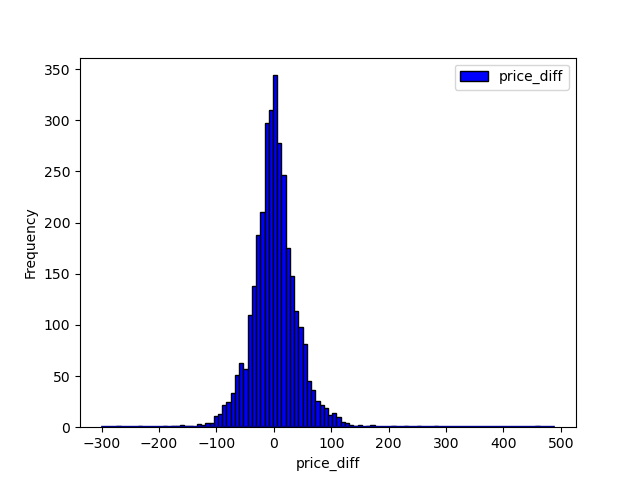
\includegraphics[scale=0.75]{/Users/janzaloznik/Desktop/Faks/magisterij/1.letnik/GEN-I/machine-learning-price-prediction-for-hourly-blocks/src/data_analysis/plots/difference_dist.png}
    \caption{Razlika med ceno na dnevnem in znotraj dnevnem trgu}
    \label{fig:Razlika}
\end{figure}

Podobno tudi ob pregledu spremembe v procentih, kjer so zaradi možnih zelo majhnih vrednosti (spremembe privedejo do ekstremnih procentov) odstranjene izstopajoče vrednosti glede na interkvartilni razmik.

\begin{figure}[h]
    \centering
    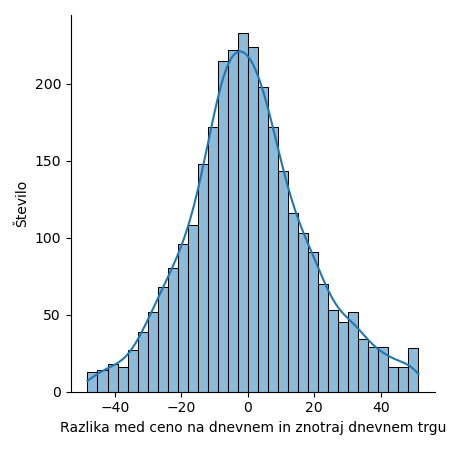
\includegraphics[scale=0.75]{/Users/janzaloznik/Desktop/Faks/magisterij/1.letnik/GEN-I/machine-learning-price-prediction-for-hourly-blocks/src/data_analysis/plots/percentage_dist.png}
    \caption{Razlika med ceno na dnevnem in znotraj dnevnem trgu}
    \label{fig:Razlika}
\end{figure}

\pagebreak
Tako lahko predpostavimo, da je cena na dnevnem trgu primerna za uporabo napovedi cene na znotraj dnevnem trgu.

Če zelo poslošimo model in uporabimo le eno ceno namesto posamičnih cen, bomo najverjetneje podcenili dejansko tveganje trgovanja, kar je razvidno na grafu, ko sta cena na dnevnem trgu in povprečna cena na znotraj dnevnem trgu med seboj zelo blizu, a hkrati obstaja velik razmak med minimalno in maksimalno ceno na znotraj dnevnem trgu v istem časovnem obdobju.

\begin{figure}[h]
    \centering
    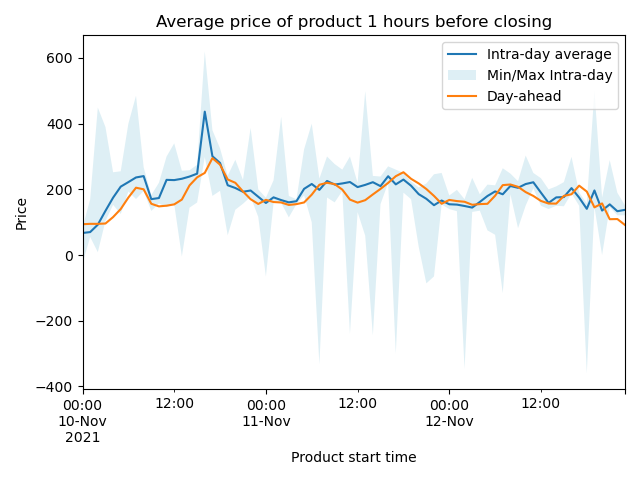
\includegraphics[scale=0.75]{/Users/janzaloznik/Desktop/Faks/magisterij/1.letnik/GEN-I/machine-learning-price-prediction-for-hourly-blocks/src/data_analysis/plots/average_price_2021-11-10-2021-11-12-mNone-MNone-hours.png}
    \caption{Razlika med ceno na dnevnem in znotraj dnevnem trgu}
    \label{fig:Razlika}
\end{figure}

Zato namesto tega napovedujemo povprečne cene posamičnih produktov znotraj časovnega intervala nekaj časa pred zaprtjem trgovanja s tem produktom.


\section{Časovne vrste in modeli}

časovne vrste so nizi podatkovnih točk, indeksirani oziroma navedeni v nekem časovnem vrstnem redu. 
Najpogosteje gre za nabor zaporednih točk, ki so na časovni komponenti enakomerno porazdeljeni (imajo isti časovni razmik). Gre torej za zaporedje podatkov v diskretnem času.

Analiza časovnih vrst obsega metode za analizo podatkov, tako da pridobimo smiselne statistične značilnosti. S pomočjo analiz lahko potem poiščemo model, ki se podatkom najbolj prilega in s pomočjo njega napovemo prihodnje vrednosti časovne vrste.
Skratka napovedovanje časovnih vrst je uporaba modela za napovedovanje prihodnjih vrednosti na podlagi predhodno opazovanih vrednosti.

\subsection{SARIMA}

Seasonal autoregressive integrated moving average oziroma SARIMA je razširjen model, bolj preprostega modela ARMA. Oba modela se uporabljata za napovedovanje podatkov časovnih vrst ali pa tudi samo za boljše razumevanje podatkov. Pri obeh potrebujemo stacionarnost, da lahko pridemo do čimboljših napovedi. 
Do stacionarnosti pridemo z odstranitvijo morebitnega trenda in sezonskosti, to lahko storimo na veliko načinov, najpogostejša načina sta diferenciranje (lahko tudi večkratno diferenciranje) in pa logaritmiranje (kjer moramo paziti da nimamo negativnih vrednosti).
Da preverimo stacionarnost časovne vrste lahko uporabimo Dickey–Fullerjev test (ADF), kjer ugotovimo, da so podatki stacionarni, če je $p$ vrednost manjša od 5\%. Na dobljenih podatkih potem narišemo grafe, kot so auto-correlation function (ACF) in Partial auto-correlation function (PACF), kjer lahko razberemo najboljše vrednosti 
za modela AR in MA. Pri AR tako ugotovimo, koliko prejšnje vrednosti vplivajo na naslednje, MA pa indicira regresijsko napako. Ostaneta nam še S in I iz kratice SARIMA, ki pomenita "seasonalty" in pa "integrated", kjer podamo vrednosti za sezonskost (npr. sedem dnevna, mesečna itd.) in še informacijo o tem ali smo podatke diferencirali.


Tako sva s pomočjo modela SARIMA napovedala vrednosti posameznih urnih blokov, vendar sva ugotovila, da napoved ni preveč dobra, saj nimava podatkov v enakomernih časovnih razmikih. Podatki namreč prikazujejo celotno trgovanje produktov, kar seveda ni v ekvidistančnih intervalih. 
Problem sva nato poskušala rešiti z glajenjem funkcije in vzeti enakomerni časovni razmik, vendar s tem sistem izgubi določene informacije in pripomore k slabši napovedi.
\ref{fig:Arima} prikazuje primer napovedi enega urnega bloka.

\begin{figure}[h]
    \centering
    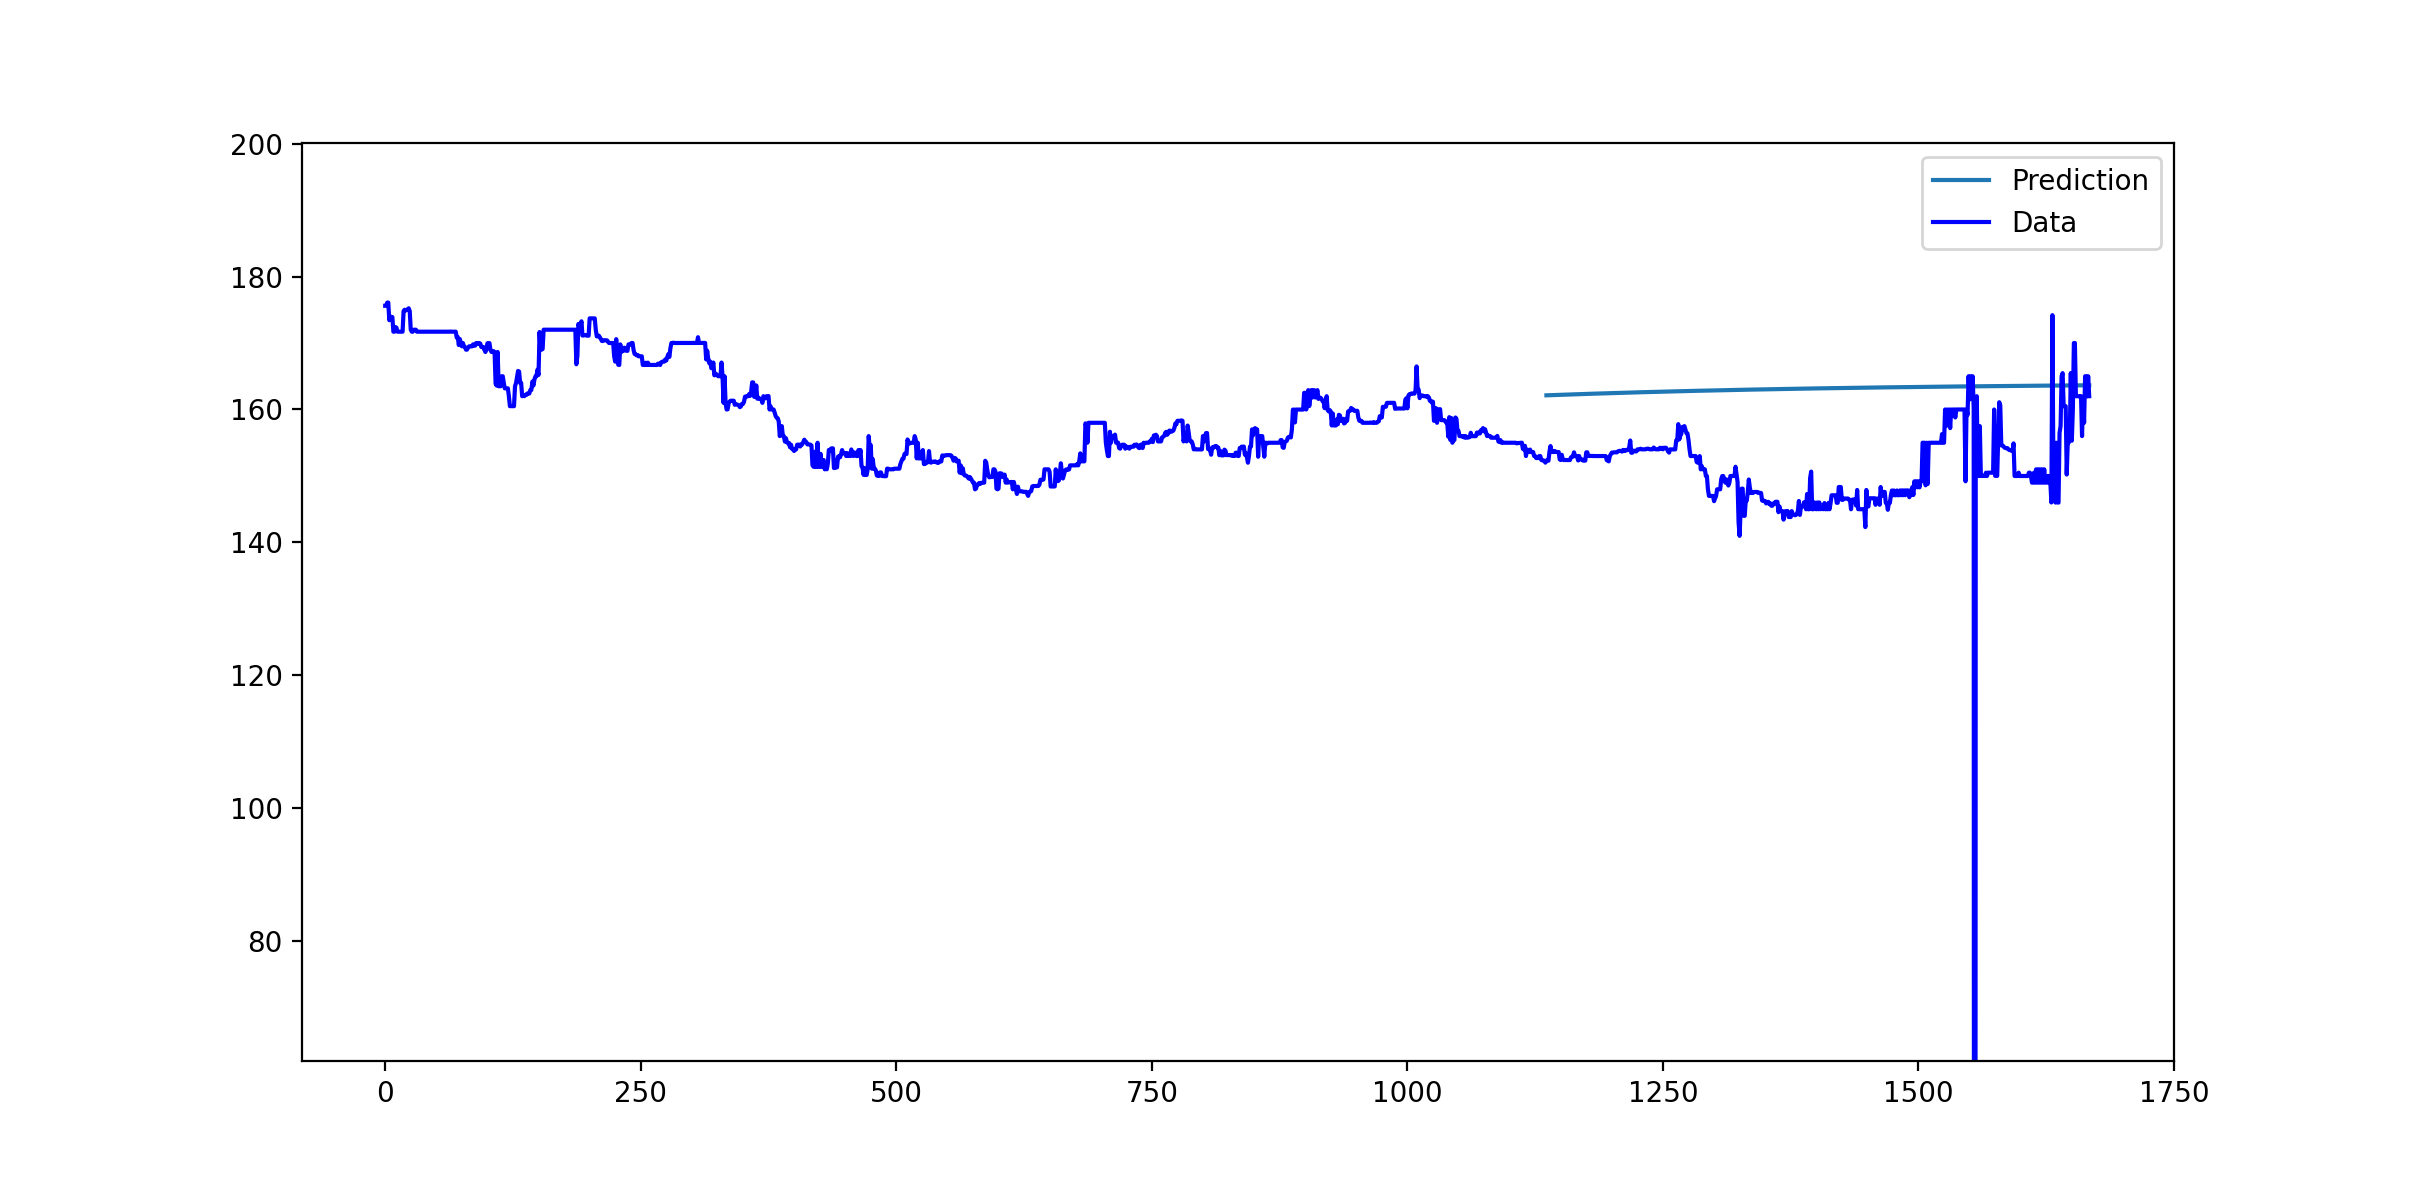
\includegraphics[scale=0.45]{Arima.png}
    \caption{Napoved za en urni blok z SARIMA}
    \label{fig:Arima}
\end{figure}



Želela sva napovedati tudi naslednjih 24 ur znotraj dnevnega trga. To sva storila tako, da sva za vsak urni blok izračunala povprečje produkta v zadnji uri. Model sva nato prilagodila glede na te podatke in dobila sledečo napoved 
\ref{fig:Prediction_intraday}.

\begin{figure}[h]
    \centering
    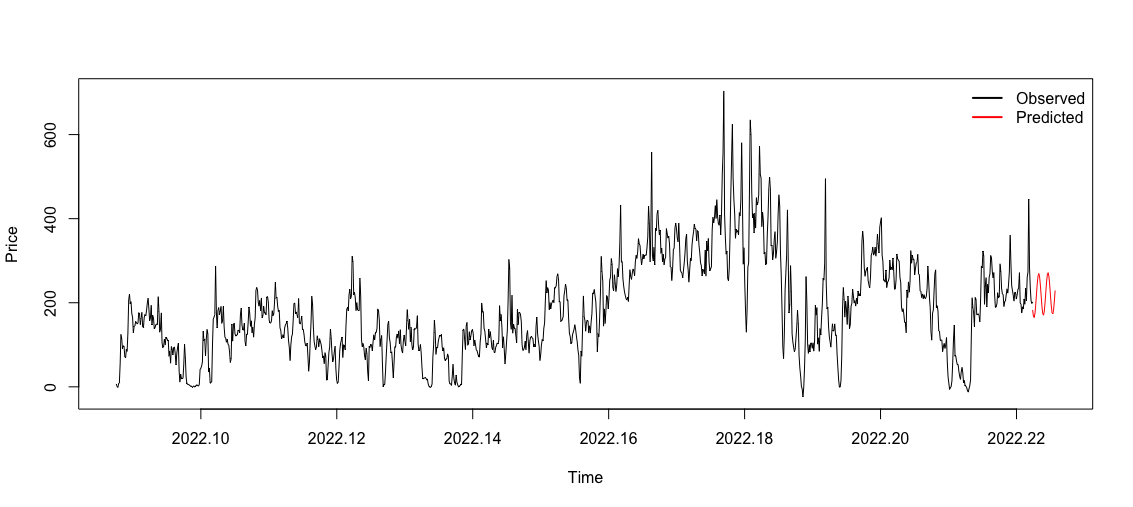
\includegraphics[scale=0.35]{Prediciton_intraday.png}
    \caption{Napoved 24 ur vnaprej na trgu znotraj dneva}
    \label{fig:Prediction_intraday}
\end{figure}



\subsection{Prophet}

Facebook Prophet oziroma Prophet je model za napovedovanje vrednosti različnih časovnih vrst. Prednost tega modela je, da stacionarnost ni pogoj za uspešno napoved, prav tako ni potrebno, da ima časovna vrsta enakomerne časovne razmike.
S pomočjo Proheta sva prav tako poskušala napovedati zadnje vrednosti urnih blokov. Kot zanimivost sva tudi primerjala napoved v času vojne (februar 2022), kjer je bila volatilnost na trgu veliko večja, in pa napoved v "normalnih" razmerah.
Ker si želiva tudi praktično koristnost najinih metod, sva se bo metoda učila na preteklih podatkih do dve uri pred koncem trgovanja za posamezni urni blok. Tako nam še ostane dovolj časa da na trg vstopimo z kratko oziroma dolgo pozicijo.
Ker bi bilo možno, da zelo oddaljeni podatki o trgovanju za določen urni blok vplivajo negativno na napoved, sva naredila tudi to primerjavo \ref{table:februar_war} in \ref{table:november_normal}. % Še sliko da nardim da se vidi 

\begin{table}[]
    \resizebox{\columnwidth}{!}{%
    \begin{tabular}{|c|c|c|c|c|c|c|c|c|c|c|c|c|c|c|}
    \hline
    Urni zamiki (X-2)           & 3     & 3,5   & 4     & 4,5   & 5     & 5,5   & 6     & 6,5   & 7     & 7,5   & 8     & 8,5   & 9     & 30    \\ \hline
    Absolutna napaka            & 76,28 & 71,45 & 67,14 & 64,80 & 62,62 & 61,71 & 60,67 & 59,79 & 59,06 & 58,27 & 57,72 & 57,23 & 56,56 & 50,86 \\ \hline
    Prophet interval (\%)       & 85,94 & 81,68 & 76,05 & 72,37 & 67,67 & 62,08 & 57,29 & 53,85 & 49,79 & 47,52 & 42,79 & 40,45 & 37,77 & 16,84 \\ \hline
    10 procentni interval(\%)   & 19,78 & 20,25 & 21,59 & 21,74 & 22,67 & 22,90 & 23,32 & 23,82 & 23,64 & 25,23 & 25,62 & 25,71 & 25,96 & 27,27 \\ \hline
    20 procentni interval (\%)  & 36,53 & 38,65 & 40,00 & 41,39 & 41,39 & 41,19 & 41,94 & 43,12 & 43,67 & 44,34 & 45,22 & 45,81 & 45,64 & 49,95 \\ \hline
    30 procentni interval (\%)  & 50,84 & 52,43 & 53,27 & 55,41 & 57,09 & 57,38 & 57,88 & 58,55 & 59,26 & 59,68 & 59,29 & 59,71 & 59,88 & 63,55 \\ \hline
    50 procentni interval (\%)  & 67,42 & 69,41 & 71,51 & 72,23 & 72,37 & 73,55 & 73,23 & 73,32 & 73,57 & 74,26 & 74,60 & 74,70 & 74,95 & 78,56 \\ \hline
    100 procentni interval (\%) & 83,33 & 83,86 & 85,71 & 86,56 & 87,49 & 87,91 & 88,42 & 88,67 & 88,51 & 88,85 & 89,19 & 89,02 & 89,27 & 90,90 \\ \hline
    \end{tabular}%
    }
    \caption{Tabela povprečij posameznih intervalov za 50 dni od 10. februarja 2022}
    \label{table:februar_war}
\end{table}


\begin{table}[]
    \resizebox{\columnwidth}{!}{%
    \begin{tabular}{|c|c|c|c|c|c|c|c|c|}
    \hline
    Urni zamiki (X-2)           & 3     & 4     & 5     & 6     & 7     & 8     & 9     & 30    \\ \hline
    Absolutna napaka            & 72,18 & 63,21 & 58,87 & 56,24 & 54,66 & 53,80 & 53,15 & 48,03 \\ \hline
    Prophet interval (\%)       & 91,48 & 86,07 & 78,00 & 70,25 & 60,00 & 51,41 & 45,25 & 19,41 \\ \hline
    10 procentni interval(\%)   & 22,87 & 24,43 & 26,41 & 27,33 & 28,66 & 28,58 & 28,41 & 30,33 \\ \hline
    20 procentni interval (\%)  & 40,73 & 45,45 & 47,66 & 48,66 & 49,50 & 50,91 & 51,25 & 55,41 \\ \hline
    30 procentni interval (\%)  & 56,92 & 59,93 & 63,50 & 65,33 & 65,91 & 66,41 & 67,16 & 71,41 \\ \hline
    50 procentni interval (\%)  & 74,95 & 80,06 & 82,50 & 83,25 & 83,33 & 84,66 & 85,41 & 86,50 \\ \hline
    100 procentni interval (\%) & 89,14 & 92,57 & 93,08 & 93,58 & 93,83 & 94,75 & 95,08 & 95,83 \\ \hline
    \end{tabular}%
    }
    \caption{Tabela povprečij posameznih intervalov za 50 dni od 10. novembra 2021}
    \label{table:november_normal}
\end{table}

\subsection{Orbit}

Orbit je prav tako model za napovedovanje vrednosti časovnih vrst, kjer je mogoče z dodajanjem različnih informacij možno vplivati na izboljšavo napovedi. Tega prej omenjena modela ne zmoreta.



\section{Rezultati}

Rezultate bova dodala po zadnjem sestanku z mentorjem.



\end{document}
